% GNUPLOT: LaTeX picture with Postscript
\begingroup
  \makeatletter
  \providecommand\color[2][]{%
    \GenericError{(gnuplot) \space\space\space\@spaces}{%
      Package color not loaded in conjunction with
      terminal option `colourtext'%
    }{See the gnuplot documentation for explanation.%
    }{Either use 'blacktext' in gnuplot or load the package
      color.sty in LaTeX.}%
    \renewcommand\color[2][]{}%
  }%
  \providecommand\includegraphics[2][]{%
    \GenericError{(gnuplot) \space\space\space\@spaces}{%
      Package graphicx or graphics not loaded%
    }{See the gnuplot documentation for explanation.%
    }{The gnuplot epslatex terminal needs graphicx.sty or graphics.sty.}%
    \renewcommand\includegraphics[2][]{}%
  }%
  \providecommand\rotatebox[2]{#2}%
  \@ifundefined{ifGPcolor}{%
    \newif\ifGPcolor
    \GPcolortrue
  }{}%
  \@ifundefined{ifGPblacktext}{%
    \newif\ifGPblacktext
    \GPblacktexttrue
  }{}%
  % define a \g@addto@macro without @ in the name:
  \let\gplgaddtomacro\g@addto@macro
  % define empty templates for all commands taking text:
  \gdef\gplbacktext{}%
  \gdef\gplfronttext{}%
  \makeatother
  \ifGPblacktext
    % no textcolor at all
    \def\colorrgb#1{}%
    \def\colorgray#1{}%
  \else
    % gray or color?
    \ifGPcolor
      \def\colorrgb#1{\color[rgb]{#1}}%
      \def\colorgray#1{\color[gray]{#1}}%
      \expandafter\def\csname LTw\endcsname{\color{white}}%
      \expandafter\def\csname LTb\endcsname{\color{black}}%
      \expandafter\def\csname LTa\endcsname{\color{black}}%
      \expandafter\def\csname LT0\endcsname{\color[rgb]{1,0,0}}%
      \expandafter\def\csname LT1\endcsname{\color[rgb]{0,1,0}}%
      \expandafter\def\csname LT2\endcsname{\color[rgb]{0,0,1}}%
      \expandafter\def\csname LT3\endcsname{\color[rgb]{1,0,1}}%
      \expandafter\def\csname LT4\endcsname{\color[rgb]{0,1,1}}%
      \expandafter\def\csname LT5\endcsname{\color[rgb]{1,1,0}}%
      \expandafter\def\csname LT6\endcsname{\color[rgb]{0,0,0}}%
      \expandafter\def\csname LT7\endcsname{\color[rgb]{1,0.3,0}}%
      \expandafter\def\csname LT8\endcsname{\color[rgb]{0.5,0.5,0.5}}%
    \else
      % gray
      \def\colorrgb#1{\color{black}}%
      \def\colorgray#1{\color[gray]{#1}}%
      \expandafter\def\csname LTw\endcsname{\color{white}}%
      \expandafter\def\csname LTb\endcsname{\color{black}}%
      \expandafter\def\csname LTa\endcsname{\color{black}}%
      \expandafter\def\csname LT0\endcsname{\color{black}}%
      \expandafter\def\csname LT1\endcsname{\color{black}}%
      \expandafter\def\csname LT2\endcsname{\color{black}}%
      \expandafter\def\csname LT3\endcsname{\color{black}}%
      \expandafter\def\csname LT4\endcsname{\color{black}}%
      \expandafter\def\csname LT5\endcsname{\color{black}}%
      \expandafter\def\csname LT6\endcsname{\color{black}}%
      \expandafter\def\csname LT7\endcsname{\color{black}}%
      \expandafter\def\csname LT8\endcsname{\color{black}}%
    \fi
  \fi
  \setlength{\unitlength}{0.0500bp}%
  \begin{picture}(3276.00,3276.00)%
    \gplgaddtomacro\gplbacktext{%
      \csname LTb\endcsname%
      \put(341,660){\makebox(0,0)[r]{\strut{}-800}}%
      \put(341,1092){\makebox(0,0)[r]{\strut{}-600}}%
      \put(341,1524){\makebox(0,0)[r]{\strut{}-400}}%
      \put(341,1957){\makebox(0,0)[r]{\strut{}-200}}%
      \put(341,2389){\makebox(0,0)[r]{\strut{} 0}}%
      \put(341,2821){\makebox(0,0)[r]{\strut{} 200}}%
      \put(341,3253){\makebox(0,0)[r]{\strut{} 400}}%
      \put(732,440){\makebox(0,0){\strut{} 6}}%
      \put(1251,440){\makebox(0,0){\strut{} 8}}%
      \put(1770,440){\makebox(0,0){\strut{} 10}}%
      \put(2289,440){\makebox(0,0){\strut{} 12}}%
      \put(2808,440){\makebox(0,0){\strut{} 14}}%
      \put(-165,1956){\rotatebox{90}{\makebox(0,0){\strut{}  $\Phi(r)$ (K)}}}%
      \put(1770,110){\makebox(0,0){\strut{}distance ({\AA })}}%
    }%
    \gplgaddtomacro\gplfronttext{%
      \csname LTb\endcsname%
      \put(2476,3080){\makebox(0,0)[r]{\strut{}$C_4F_{10}-C_4F_{10}$}}%
      \csname LTb\endcsname%
      \put(2476,2860){\makebox(0,0)[r]{\strut{}$C_5F_{12}-C_5F_{12}$}}%
      \csname LTb\endcsname%
      \put(2476,2640){\makebox(0,0)[r]{\strut{}$C_6F_{14}-C_6F_{14}$}}%
    }%
    \gplbacktext
    \put(0,0){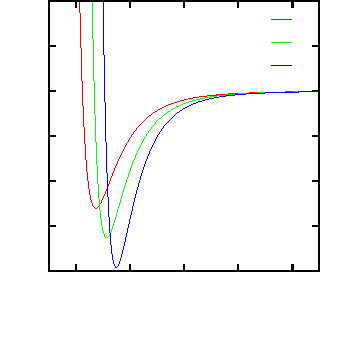
\includegraphics{c2_plot_potentials}}%
    \gplfronttext
  \end{picture}%
\endgroup
